\chapter{绪论}
\section{研究背景}
如今,计算机和互联网发展的飞速发展推动我们迎来新一轮的伟大变革——第四次工业革命,也就是工业4.0时代。工业4.0 有两大主题——智能工厂与智能生产,其实质是推动工业互联网的发展,该战略的提出凸显了全球制造业激烈竞争的态势。\par
我国是世界上公认的制造业大国,传统制造业占比大,因此工业4.0 的提出对我国传统制造业的发展提出了巨大的挑战,其迫切要求我国工业企业从劳动密集型生产模式转向高效率、高科技生产模式。因此,我国政府高度重视工业4.0 的发展,在《中国制造业发展纲要(2015-2023)》中明确指出要结合我国自身的实际情况,大力发展工业4.0,加大智能工厂、智能生产的发展,决不能只作为一个被动的追随者,要摆脱“世界加工厂”的角色,成为工业4.0 变革的引领者!因此,考虑如何将工业互联网应用于实际,快速提高工业企业的生产效率是当下迫在眉睫的问题。\par
在工业企业生产控制中,数字控制机床发挥着重要作用,其依托程序控制系统自动加工零件,其中,机床主机是自动完成零件切削加工的重要部分。而在机床主机上,刀具是关键因素。生产实践证明,机床主机上的刀具磨损后会对工厂的生产效率及产品质量造成影响。如果在刀具状态未超过磨损极限点时进行换刀操作,会造成不必要的资源浪费;若超过刀具磨损极限点未及时更换刀具,会降低机床加工质量,延误零件加工进程。因此,如果能准确预测刀具磨损程度并及时更换刀具,则可大幅提高工业企业的生产效率。\par
目前,对于刀具磨损量预测方法主要有经验判断和图像检测法。经验判断法主要由人工判断刀具磨损量或者设置固定换刀时间。该方法主观性过强,无法高效精确地预测换刀时间。而基于图像识别刀具磨损量是利用计算机识别刀具磨损的图片,进而判断磨损量。该方法需要中断加工过程,实时性低,影响加工进度。如果能够将刀具磨损数据实时输入计算机中,进而利用数学模型精确预测刀具磨损量,则可以实现在线监测,还具有相当的成本优势。考虑到刀具磨损数据具有复杂的非线性、相互耦合等特点,简单的线性分析无法有效预测刀具磨损量。相比之下,机器学习可获得大量信息,对于解决复杂非线性关系有明显的优势。\par
目前,机器学习算法能够处理高维和多变量数据,可在复杂和动态环境中提取数据的隐藏关系,其通过对计算机进行编程,利用样本数据或以往的经验来解决给定的问题。神经网络、回归模型是机器学习中常用的两种算法。其中,神经网络采用一种类似大脑神经突触联结的结构,由大量简单的处理单元连接组成,通过分布式并行信息处理算法,依靠大量的节点(神经元)之间的复杂系统,调整内部间的相互连接关系,进而处理信息,具有自学习和自适应的能力。而回归模型可预测机器还有多少时间会出现故障。为使回归模型起作用,必须提供历史数据。理想情况下,各种类型的故障都会被表示出来。其提供的假设是,基于系统的固有(静态)方面及其当前性能,可以预测其剩余生命周期。但是,如果系统发生故障的方式有多种,则必须为每种可能性创建一个单独的模型。因此,机器学习模型可收集机床传感器数据,并基于历史故障数据,识别故障之前的事件。通过预先设置所需的参数,以触发潜在故障的警报。当传感器数据超出这些参数阈值时,将启动及时换刀警报。\par
通过上述总结可得,机器学习支持以最少的人为干预,分析大量数据。通过应用机器学习,结合从传感器收集的数据,可高效、精确预测机床刀具磨损程度,进而提醒工作人员及时更换刀具,能够提高工业企业生产效率。\par
\newpage
\section{研究意义}
当前我国正处于迈向工业4.0的关键节点,传统制造业中不被重视的产品质量,现在在新生产架构下开始变得愈发重要。产品质量侧面反映一个国家的制造业水平,其中加工中心刀具磨损量对于加工品精度影响巨大。对于传统公式化的刀具磨损度测量方法所反映出的种种弊端(需要停机检查,对于工人的高素质要求,以及复杂的公式),造成刀具磨损度测量面临的阻碍,严重影响工业生产以及学术研究。我们团队试图通过机器学习这一革命性的方式,不停机进行刀具退化程度测量。 \par
我们通过机器学习测量出的加工中心刀具退化程度数据,应用场景将十分广泛:由质量与刀具磨损质量建关系可以用来优化工业企业的备件库;嵌入工业软件中用于刀具健康状况警报,提醒工人及时更换刀具等。\par
通过刀具磨损量预测模型,一方面可使机床刀具利用率最大化,减少工厂资源浪费,提高工作效率;另一方面,通过预测模型可有效预防刀具报废带来的损害,及时控制成本。对刀具备件库存进行优化,可减少不合理的备件库存量,降低储存成本;同时,可为工厂制定合理的库存操纵策略提供有效指导。\par
% 
% 
\subsection{传统刀具磨损量测定存在的问题}
数控加工中心的刀具磨损情况,对于加工件的质量(如:表面粗糙度与尺寸公差)有很大影响,如果能对机床的车刀磨损量有一个相对准确的测定,同时根据磨损量与质量间的关系确定更换机床刀具的时间,将能极大提升机加工产品的质量。\par
在工业界,对于刀具磨损量测定主要有以下两个方法:(1)高级工程师的经验与传统机械公式判断:该方法中经验公式的系数由大量数据总结而成,但是针对不同刀具公式变化频繁,且有经验的工程师培养周期很长;(2)基于图像识别的刀具磨损量检测:该方法利用卷积神经网络输入海量标注磨损度的刀具数据,对这些数据进行训练,但是其需要人力去标注数据,且图像识别精度有限,测定值与实际磨损存在较大偏差。\par
同时,以上2种刀具磨损量预测方法都存在一个对于实际生产影响巨大的问题:需要停机并且人工清理好切屑才能进行检验,绝大多数机加工企业的流水线生产对于流水线连续性要求很高,停机检查会让整个生产周期拉长。\par
% 
\section{方案总体研究框架}
在确定研究课题后,我们通过文献研读,进行了实际调研、机床分析、搜集数据三方面的工作。在此基础上,我们对机床刀具切削数据进行分析处理,总结得到对刀具磨损量预测与实际偏差较大。为此,我们利用反向传播神经网络预测刀具磨损量,在此基础上,对刀具备件库存进行优化(图1.1论文总体研究路线)。\par

\begin{figure}[htp]
    \centering
    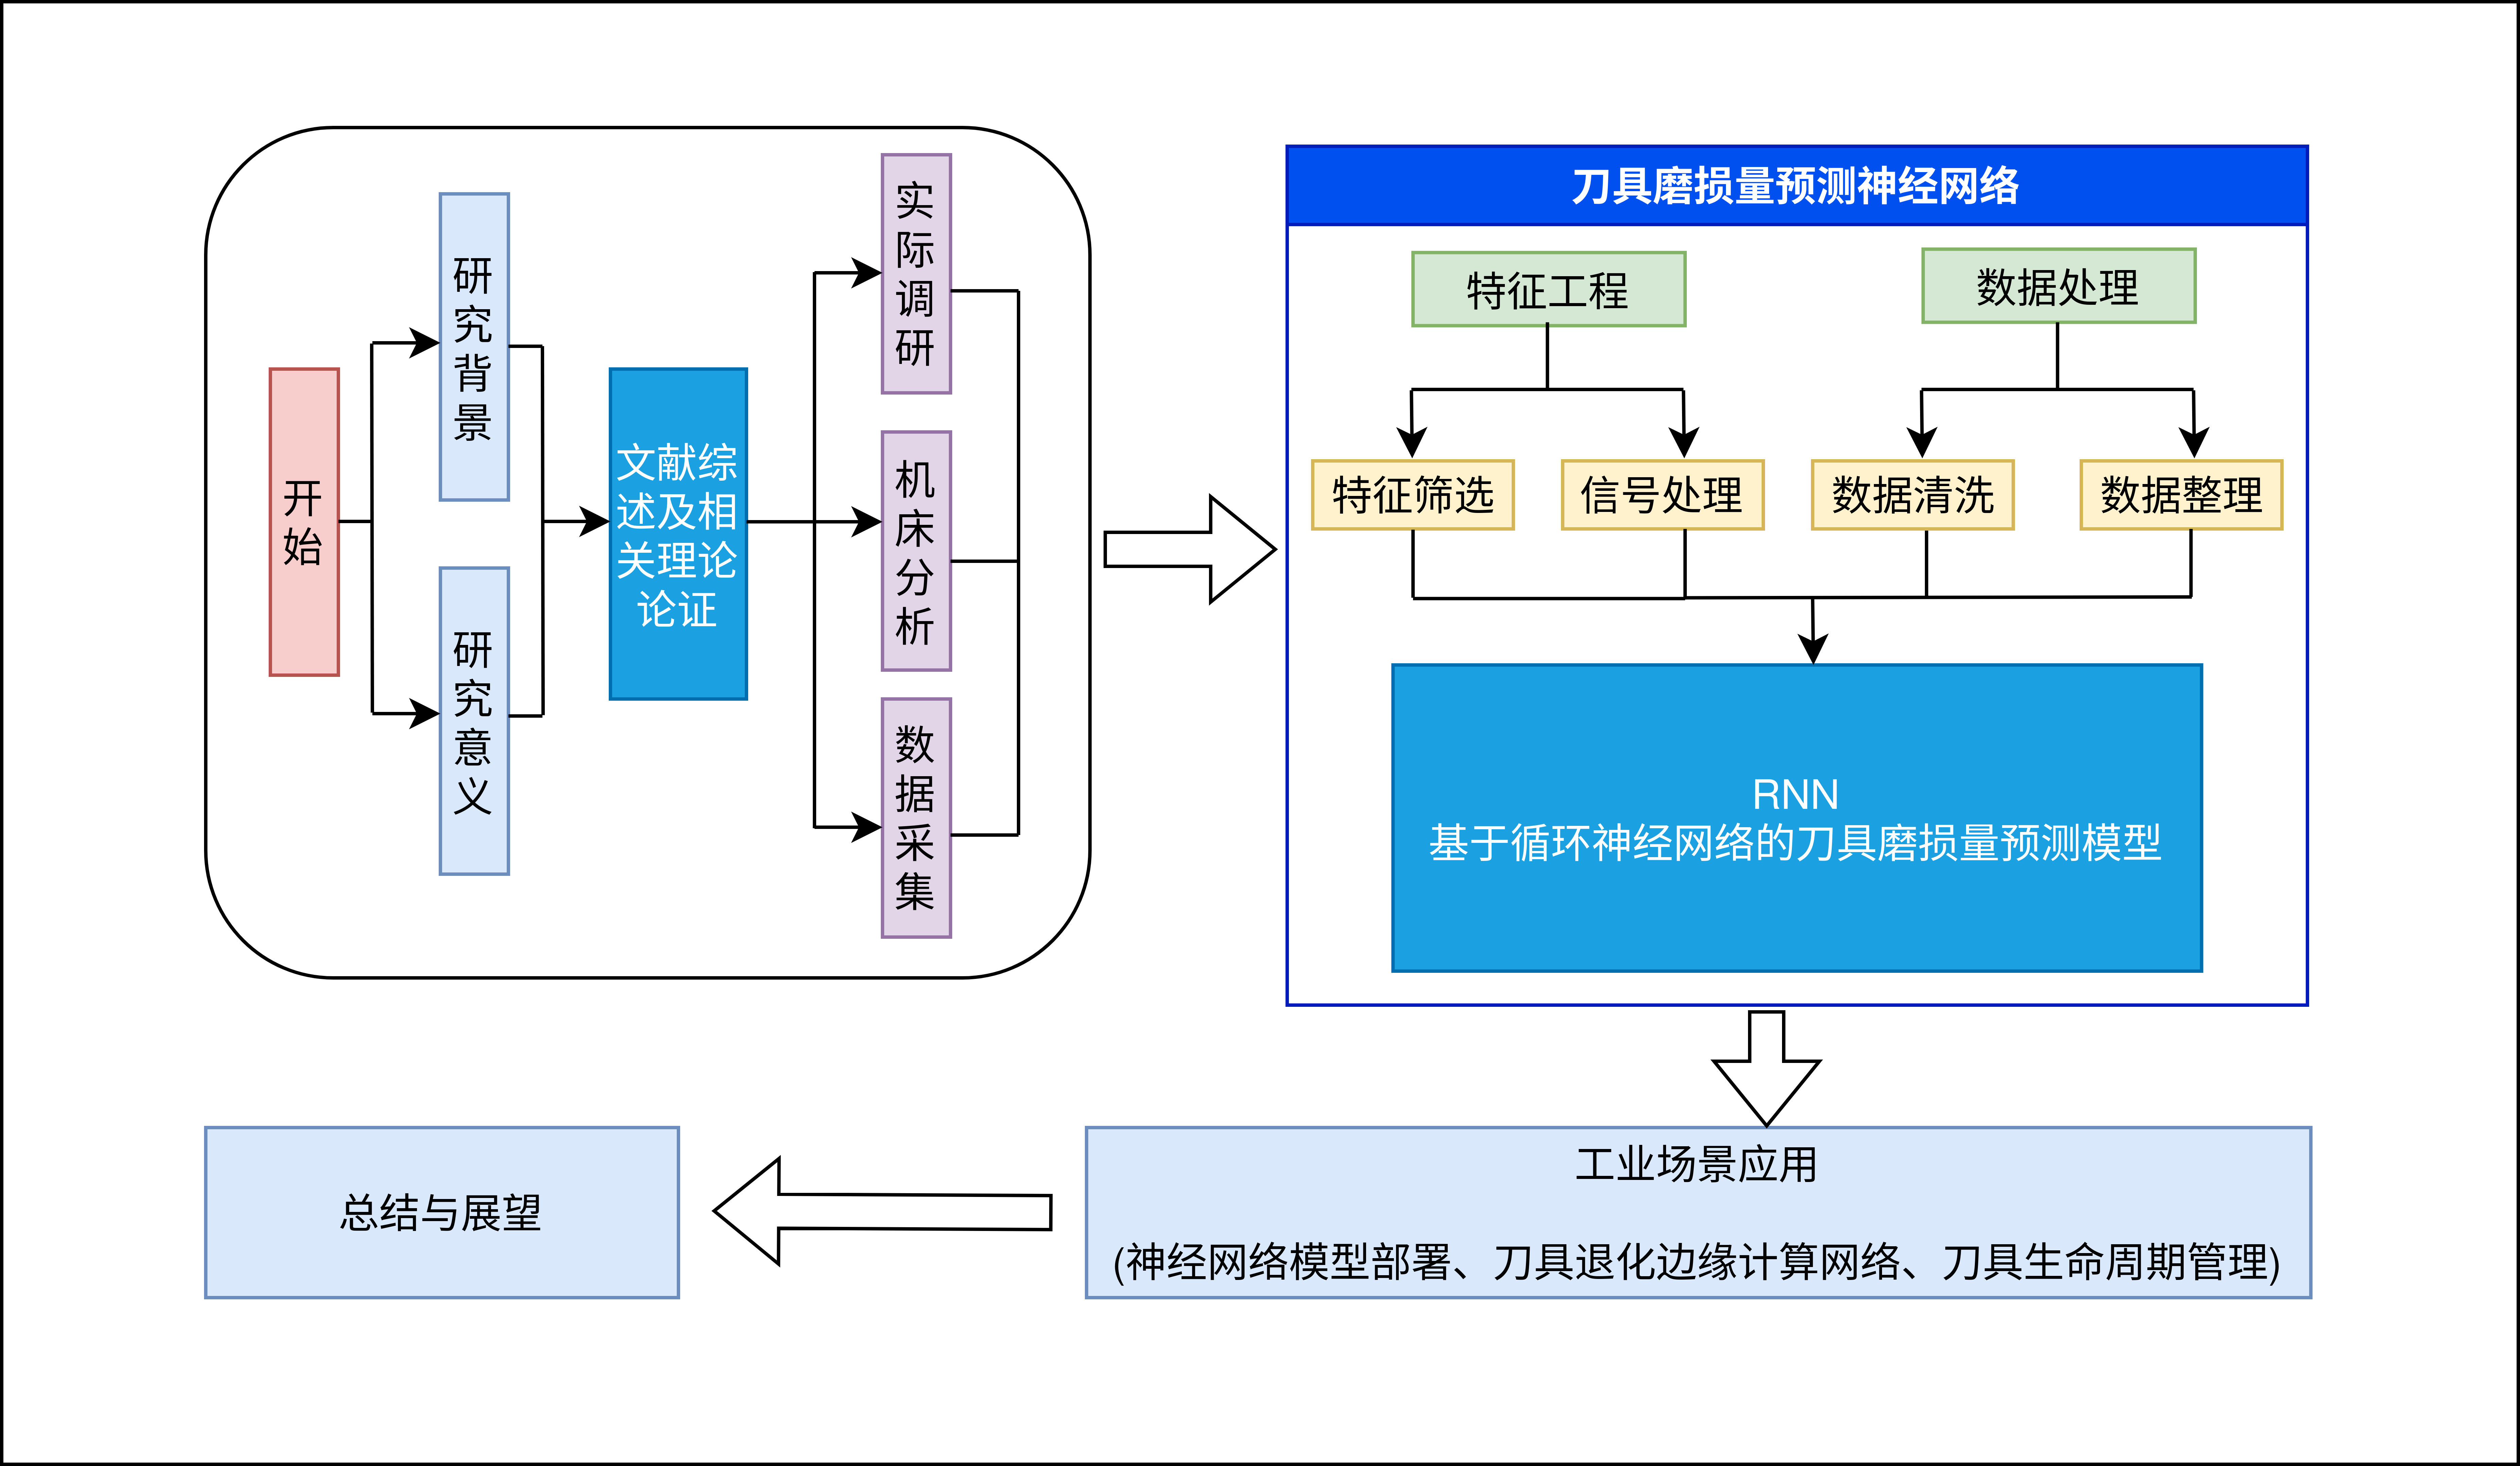
\includegraphics[width=14cm]{Chapter1/OpenIE研究架构.png}
    \caption{论文总体研究路线}
\end{figure}

% \begin{figure}[htp]
%     \centering
%     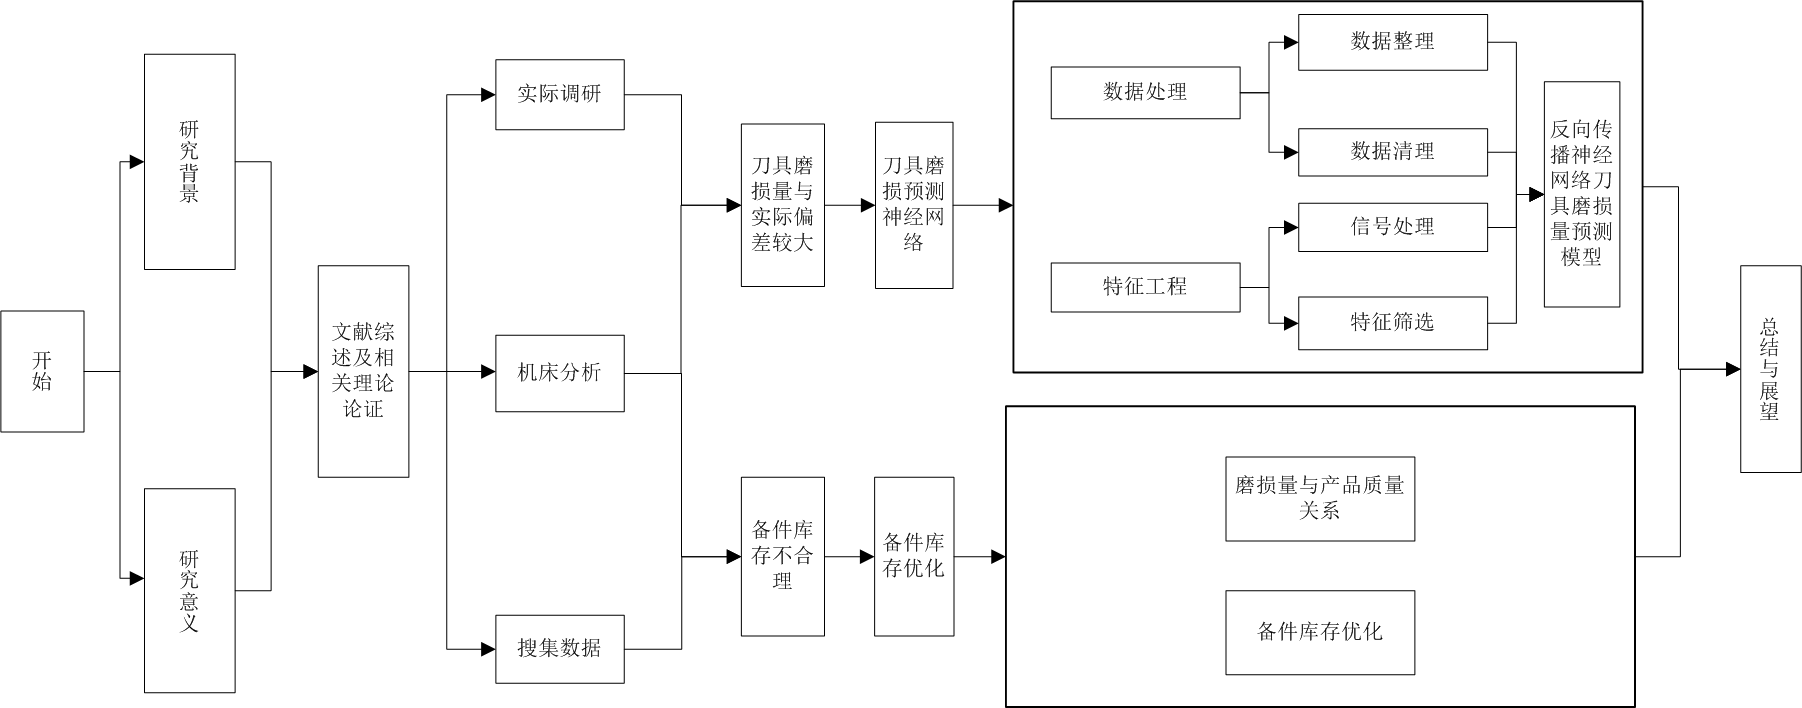
\includegraphics[width=14cm]{Chapter1/全文流程图.png}
%     \caption{方案总体研究框架}
% \end{figure}
